
%%% Local Variables: 
%%% mode: latex
%%% TeX-master: t
%%% End: 

\chapter{图像预处理与环结构}
\label{cha2}

\section{预处理}
 因硬件条件的限制,采集图像通常存在着血管与背景对比度低、照度不均匀、大量噪声点分布等问题,这大大增加了自动识别分析的难度。因此,我们需要对其做适当的预处理,以便于提取视网膜图像重要的血管特征,用于下面的配准工作。预处理工作主要由基于多小波核和多尺度的分割方法~\cite{wang},阈值去噪、填充空洞和骨架化步骤组成。经过这几步处理,最终得到了单像素的灰度图像用于下步的环结构提取。
\subsection{多尺度分割}
在我们的工作中,选择了基于多尺度和多小波核的视网膜血管分割方法用来进行多尺度的血管分割~\cite{wang}。这种方法预先不需要对视网膜图像预处理与训练,因此能直接用于用于不同特征的图像集。同时它采用自适应的阈值方法,而不需要人工进行参数的调整。
它的主要步骤是:
 \begin{enumerate}
\item 利用多小波核的对应滤波技术(MFMK)处理杂乱的血管边缘,明亮的局部特征等问题,得到增强后的视网膜图像。
\item 为解决图像噪声去除和血管正确定位的问题,对归一化的增强图像应用多尺度分层的分割方法。多尺度分层分割方法是一个迭代的分割过程,每一次迭代图像的分辨率增强,能够定位到的血管越来越小。这个过程是由一个简单的尺度参数控制的,它控制了血管细节的程度,血管的信息都储存在血管图中。同时通过一个必要条件确定最优分割结果及尺度。
\item 基于前面过程提取的血管边缘信息确定阈值平面,并通过局部自适应阈值得到最终的血管二值图像。
 \end{enumerate}
 
图~\ref{multiscale}显示了一幅视网膜图像及对应的几个尺度的分割结果。
 \begin{figure}
\centering
\begin{minipage}[b]{0.45\linewidth} 
      \centering 
      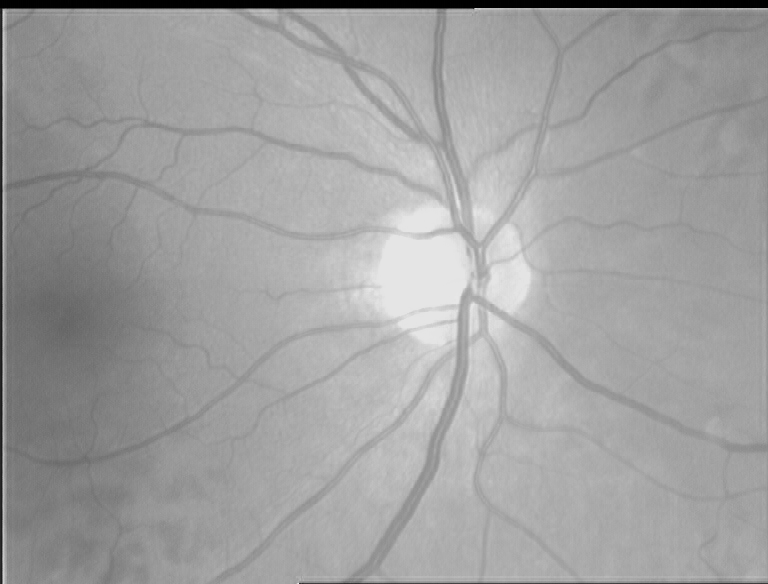
\includegraphics[width=0.9\linewidth]{R096.png}
        \centerline{(a) }\medskip
\end{minipage}
  \begin{minipage}[b]{0.45\linewidth}
    \centering
    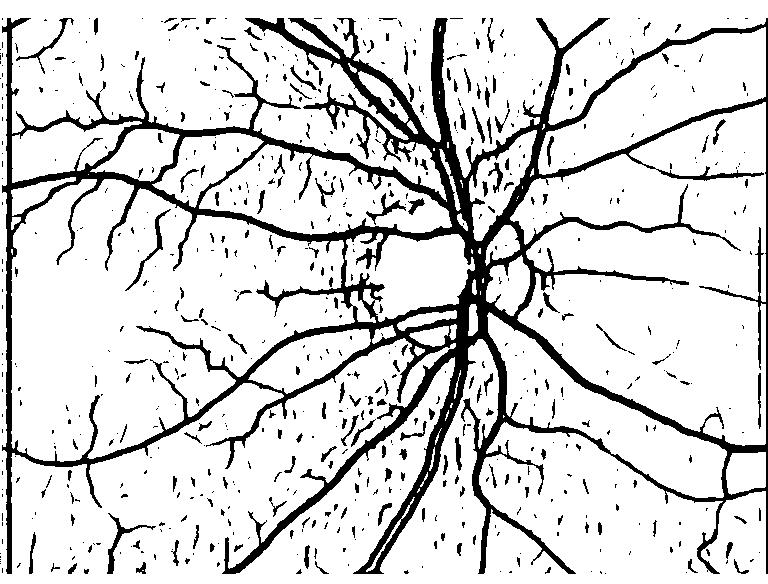
\includegraphics[width=0.9\linewidth]{R096-03.jpg}
      \centerline{(b) }\medskip
  \end{minipage}
    \begin{minipage}[b]{0.45\linewidth}
    \centering
    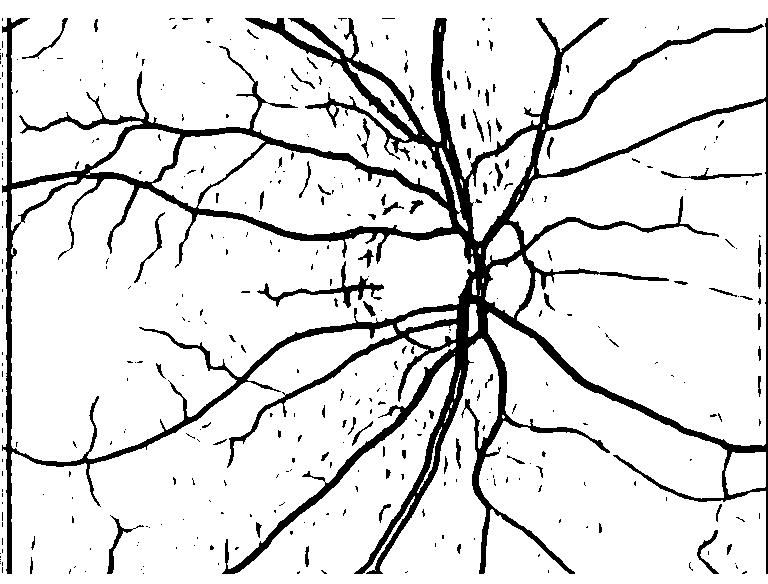
\includegraphics[width=0.9\linewidth]{R096-07.jpg}
      \centerline{(c) }\medskip
  \end{minipage}
  \begin{minipage}[b]{0.45\linewidth}
    \centering
    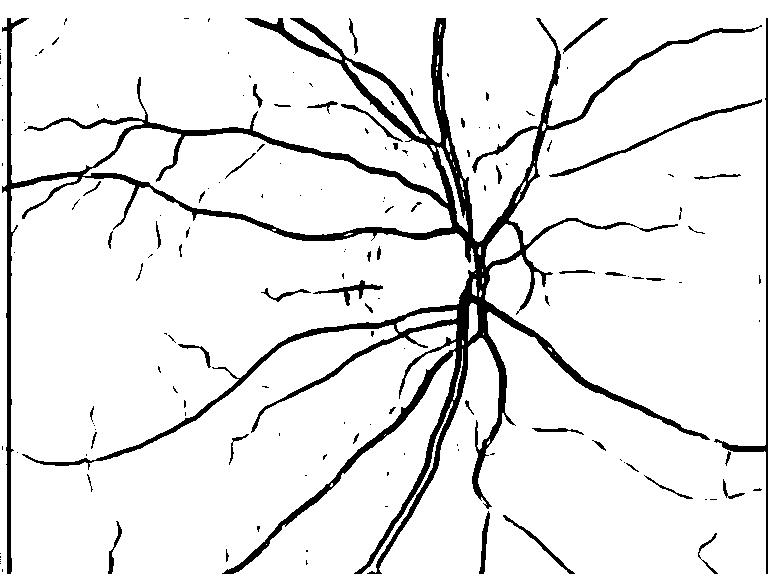
\includegraphics[width=0.9\linewidth]{R096-09.jpg}
      \centerline{(d) }\medskip
  \end{minipage}
 \caption{一幅视网膜图像及对应3个尺度的分割结果}
\label{multiscale}
\end{figure}

由图~\ref{multiscale}分割结果可以观察到,从图$(a)$到图$(b)$,分割出来的血管数量逐渐增多,一些细小的血管也逐渐分割出来,但同时噪声也在增加。随着分割层数的增加,提高了噪声增加的概率。在~\cite{wang}提出的多小波核和多尺度分层分割中,为了降低噪声,同时最大程度的保留血管细节,通过使信噪比(SNR)最大,可以得到最优分割结果同时得到相应的尺度参数值。图像的信噪比一般为信号与噪声的功率谱之比,但我们通常用信号与噪声的方差之比近似估计图像信噪比。 

不同尺度的分割结果代表不同程度的细节信息,在实际视网膜图像中构建环结构需要较丰富的血管细节信息,同时也要排除噪声的干扰,我们很难判断哪个尺度的分割结果可以有利于得到我们的环结构,而单个最优尺度分割结果不一定适合我们环结构构建的要求。因此在本文中,我们选择不同图像分辨率下的14个尺度的血管分割二值图作为下一步处理的分割图,可以有效避免因单个尺度的分割结果不理想造成的特征提取失败。后续我们会通过一系列处理选出最优配准结果对应的尺度。

\subsection{连通区域标记法去噪}
在分割后的多个尺度的图像中存在着噪声,这对环结构的提取造成了困难,本文中我们采用连通区域标记方法对图像进行去噪。连通区域标记是在计算机视觉和图像分析处理的众多应用领域中较为常用的方法,它首先标记二值图像中所有的目标像素,由此形成多个被标示的连通区域,然后我们在此基础上获取这些区域的轮廓、质心、不变矩等几何参数,在一些需要将前景目标提取出来以便进行后续处理的应用场景中常能够用到连通区域分析方法。通常连通区域标记方法处理的对象是二值化后的图像。常用的连通区域标记法有两遍法、种子填充法等。

连通区域一般是指图像中具有相同像素值且位置相邻的前景像素点组成的图像区域。我们可以通过这个定义在图像中找到连通区域,给它们每一个赋予一个唯一的标示(Label),如1、2、3$\ldots$,以区别其他连通区域。根据像素相邻关系的不同,可以分为4连通标记、8连通标记,如下图 ~\ref{liantong}所示。
   \begin{figure}[ht!]
   \centering
  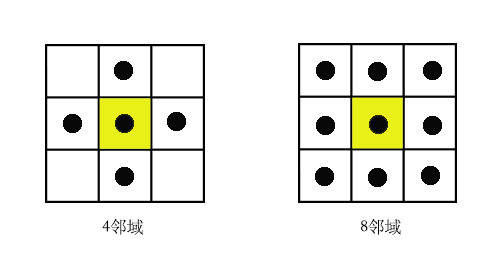
\includegraphics[width=0.8\linewidth]{4-8邻域2.png}
  \caption{4邻域与8邻域图示}
   \label{liantong}
 \end{figure}
 
4连通是指如果有两个像素,其中一个像素的位置在另一个像素的上、下、左、右,就判定这两个像素是连通的;8连通则是说一个像素的位置在其他像素相邻的上、下、左、右、左上角、左下角、右上角或右下角,则认为它们是连通的。本文采用8连通区域标记。

在将多尺度分割后分割后的视网膜图像通过连通区域标记后,我们将像素个数小于阈值的连通区域判定为非血管进行去除。通过滤除噪声,可以有效降低对后续骨架化和寻找环结构的干扰。

\subsection{空洞填充和骨架化}
通过对分割后图像的观察,我们可以看到分割出的血管有时会出现中空的现象。这是由于视网膜图像的动脉和静脉血管在拍摄时出现中心光线反射~\cite{hari}造成的。中心反射现象更易出现在血管氧气丰富,尤其是光照比静脉略有不足的动脉上。它会使一条血管出现两条痕迹,在下一步的骨架化中被误认为两条血管,从而对于配准准确性产生影响。

因此我们采用传统的先膨胀、再腐蚀方法对多尺度分割图像进行操作以填充孔洞。膨胀、腐蚀是图像形态学中常见的操作方法。由图 ~\ref{ske-fill}可以看出,经过膨胀、腐蚀后的血管空洞得到了填充,这样在骨架化的时候就会正确的识别为一条血管,保证了骨架化的正确性。
   \begin{figure}[ht!]
   \centering
 \begin{minipage}{0.45\linewidth}
  \centering
  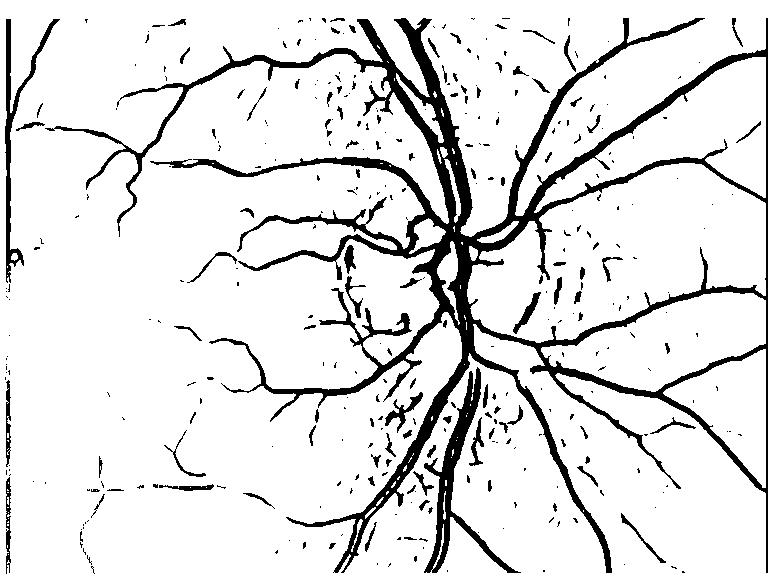
\includegraphics[width=\linewidth]{119-11.jpg}
\end{minipage}
\begin{minipage}{0.45\linewidth}
  \centering
  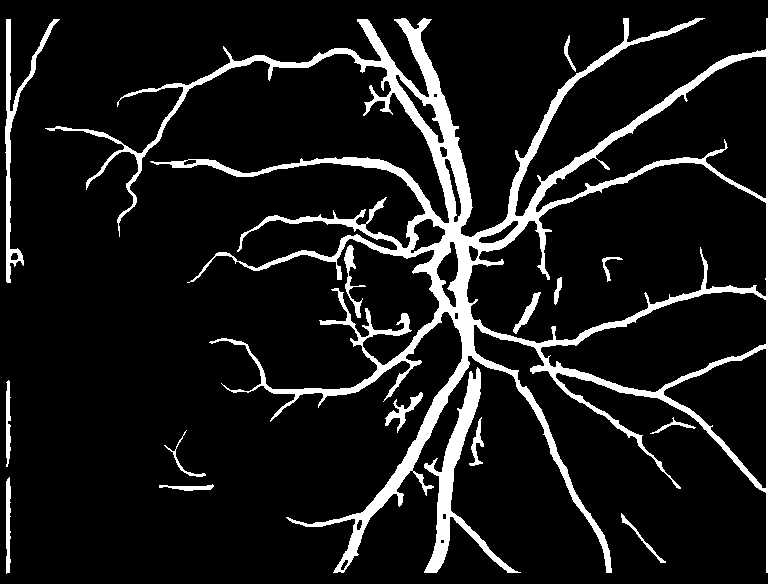
\includegraphics[width=\linewidth]{119-11.png}
\end{minipage}
  \caption{分割图像与填充后图像对比}
    \label{ske-fill}
 \end{figure}
最后我们对经过膨胀腐蚀处理后的血管进行骨架化操作以得到单像素宽度的血管树,这里采用的是Nicholas R. Howe\footnote{http://www.cs.smith.edu/$\sim$nhowe/research/code/}实现的轮廓修建骨架化方法,是由Alex Telea提出。这个方法的主要思想是:将骨架上的一个点看做一个圆的中心,这个圆在多个点碰触图像的边缘。灰度骨架化图像的灰度值是基于沿着图像的周长连接最远距离的两点的最短距离,骨架上由于小的边缘扰动形成的毛刺则会有较小的灰度值,即使它们很长。如果圆碰触到两个不连续的边(如O型的内外),则骨架化在那个点是一个无限的过程。为了得到最终的骨架化结果,应该根据轮廓的噪声突出的预期大小来选择阈值。骨架是一种更为简洁、明了的表示方法,它不仅充分显示了视网膜血管的轮廓信息,还能够保持视网膜的拓扑属性,对于后续的处理也更有优势。图 ~\ref{ske}显示了最终的骨架化结果,经过了骨架化处理,视网膜血管的大体轮廓及血管细节可以清晰的观察到。
    \begin{figure}[ht!]
   \centering
  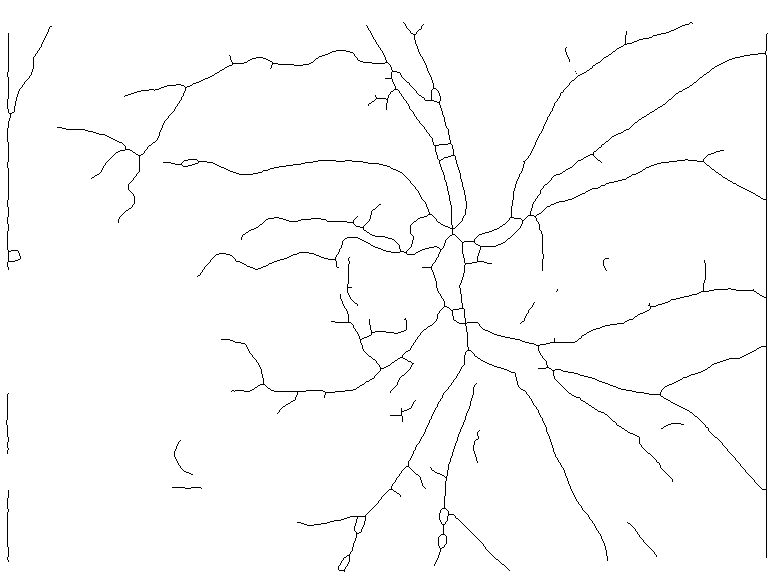
\includegraphics[width=0.5\linewidth]{119-ske-11-new.png}
  \caption{与图  ~\ref{ske-fill}对应的最终的骨架结果}
    \label{ske}
 \end{figure}
 
 我们将视网膜配准的参考图像与待配准图像都进行了上述的多尺度分割,去噪,血管填充和骨架化处理,最终分别得到了14个血管骨架化结果(参考图像的每个$N_j,j=1,2,\ldots,14$需要与待配准图像的每个$M_i,i=1,2,\ldots,14$进行一一对齐),下一步我们将进行环结构的寻找。
 
 \section{配准特征简述}
 \subsection{点匹配特征}
 为了完成后续的坐标变换,我们必须首先选择合适的视网膜特征。众所周知,对于基于特征的配准方法来说,只要采用足够鲁棒的特征,配准的精度会大大提高。而特征匹配的准确度越高,对于后续的变换模型的参数估计越加有利。一个好的特征应该对不同的变换模型保持特征不变性,在噪声的条件下仍然保持足够的鲁棒性。我们观察视网膜图像得知,最重要的特征便是其血管网络及有血管组成的分支结构。而对于视网膜的血管和分叉点作为特征在配准中的应用,都有大量的学者对此进行了广泛的研究。
 
关于血管的特征提取方法,大概分为两种:一种为像素处理方法,先对图像进行自适应滤波或分割,再进行收缩或分叉点分析以得到血管的骨架图。这种方法需要对每个图像像素进行处理和操作。另一种为血管追踪算法,它的过程是:首先定位一个初始点,然后利用每个图像像素的局部图像性质去迭代的追踪血管。提取到的特征是沿着血管中心线的追踪点,最终的结果是血管的中心线。它仅仅处理与血管相似的像素,避免了对每个图像像素的处理,因此也被称作“探索性算法”。这种方法的缺点是易被血管的灰度值的不连续性或血管的断裂影响。 
 
虽然血管对几何形变和灰度值的改变足够鲁棒,但其本身并不适合作为一个配准的特征,通常将求取视网膜血管作为进一步提取配准结构的预处理,如上述的两种方法都可以作为求取分叉点的预处理步骤。
 
 对于分叉点来说,它们广泛存在于在视网膜图像中,也是人眼观察视网膜图像易观察到的重要特征,因此分叉点结构是一个得到广泛使用的配准特征。为了使分叉点在配准时更加唯一,我们需要采用一些不变的特征来标识分叉点,易观察到分叉点的各个分支的角度是不随着平移,旋转,缩放而改变的,因此可以作为标识分叉点的合适的选择。图~\ref{bifur}为一个带有三个分支角度的分叉点实例。
   \begin{figure}[ht!]
   \centering
  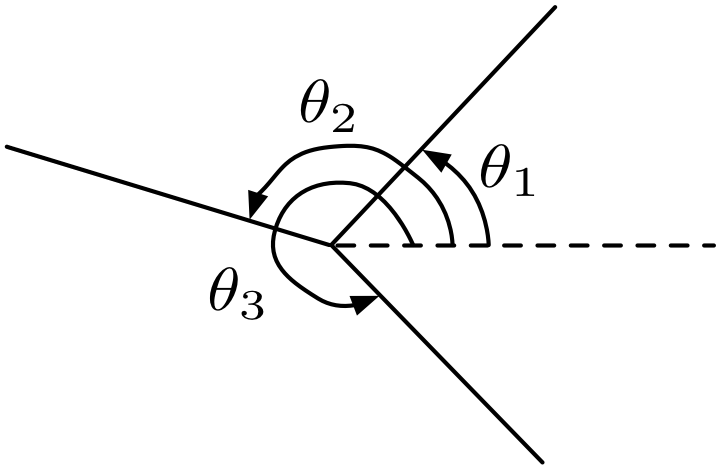
\includegraphics[width=0.45\linewidth]{分叉点.png}
  \caption{一个带有三个角度的分叉点实例}
    \label{bifur}
 \end{figure}
 
 在文献~\cite{zana}中,为了找出参考图像与待配准图像的对应的分叉点,提出了以下的度量方法:
 \begin{equation}
 d(M^{'},\theta_i)=\inf_{j=1\ldots4,k=-1\ldots1}\{|\theta_i-\theta_j^{'}|+2k\pi\}
 \end{equation}
 其中$M$和$M^{'}$是两幅图像上对应的点,$\theta_i$和每个$\theta_j^{'}$由单位圆上的一点表示,$d(M^{'},\theta_i)$等于从到离他最近的点之间的弧度。其中,$M$和$M^{'}$的距离定义如下:
  \begin{equation}
 d(M,M^{'})=\inf\Big\{\sum_{i=1}^4d(M^{'},\theta_i);\sum_{j=1}^4d(M,\theta_j^{'})\Big\}
 \end{equation}
 
 实际上为分叉点和之间的相似性度量。然后采用贝叶斯霍夫变换和仿射参数估计,选择最优变换参数来完成配准。
然而,分叉点结构若只使用角度来标识本身特性作为配准特征,有如下不可忽视的缺点:分叉点分支间的角度不具有唯一性,对一幅视网膜图像来说存在许多个分叉点,分叉点的分支角度都极为相似,这就使得在求取对应特征分叉点时极易造成错配,因此对于配准目的来说不够可靠。
 
在~\cite{stewart}中,作者提出了基于分叉点的landmark结构。每个landmark由一个分叉点,该分叉点的三个血管分支的方向角度,以及对应的血管的宽度组成。其中方向角度的差值(即该分支的分支角度)和血管宽度的比率对于图像的平移,旋转,缩放是不变的。因此一个landmark的不变的signature特征由分叉点的分支角度及血管宽度比率组成,共6个变量,如图~\ref{landmark}所示。该不变的signature特征向量用来做两个分叉点的相似性度量,每个signature特征向量都能找到与之最近的匹配,然后当signature特征向量间的马氏距离在95$\%$的置信卡方不确定性边界内时,确定最终的匹配特征向量。
  \begin{figure}[ht!]
   \centering
  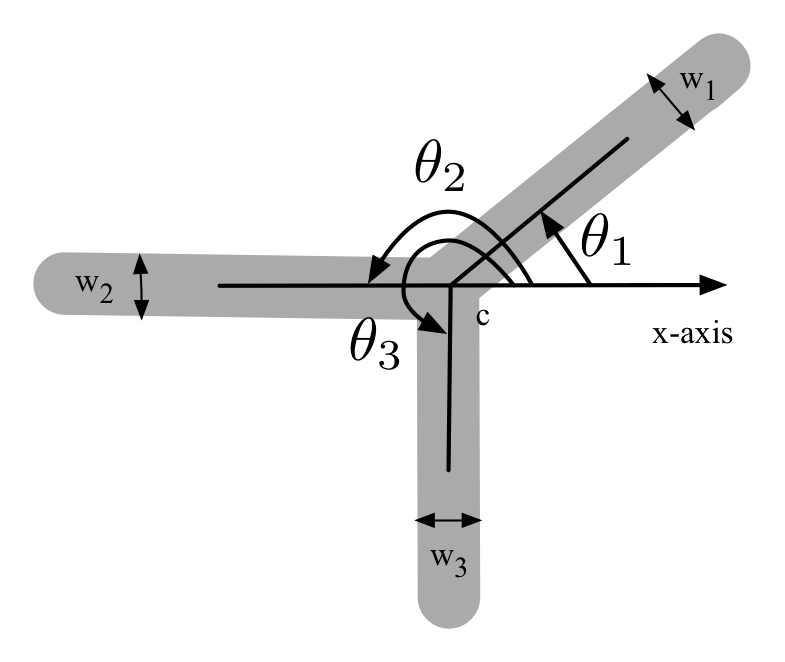
\includegraphics[width=0.45\linewidth]{landmark.png}
  \caption{landmark图示}
    \label{landmark}
 \end{figure}
 
上述为传统的依据分叉点作为配准特征的情况,考虑到单纯的分叉点结构逐渐无法满足日益准确的配准结果的要求,学者们又做了许多研究的工作,将配准的特征从以往简单的基于点配对的技术,转换到基于结构的配准方法,更多的考虑到了视网膜整体的结构特征。
 
 \subsection{结构匹配特征}
 Chen等人~\cite{chen}提出了一种新的结构特征来进行视网膜图像配准,也就是所谓的bifurcation结构。一个bifurcation结构由一个主分叉点和它的三个邻域分叉点组成,如图~\ref{bifurcation}所示。
   \begin{figure}[ht!]
   \centering
  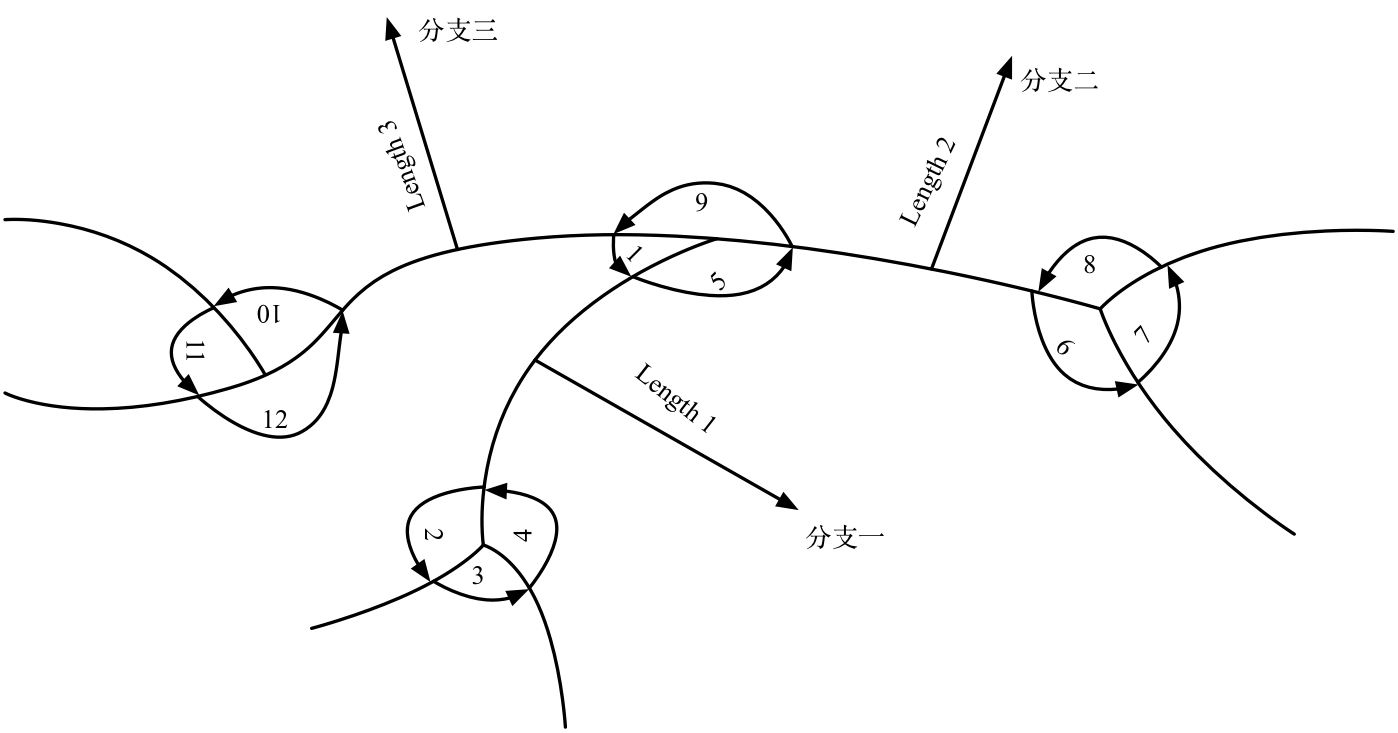
\includegraphics[width=0.8\linewidth]{bifurcate.png}
  \caption{Bifurcation结构示意图}
    \label{bifurcation}
 \end{figure}
 
 上述bifurcation结构的主分叉点有三个邻域分支,其长度编号分别为1,2,3而角度的编号为1,5,9,而每个分支与一个邻域的分叉点相连。该bifurcation结构的特征向量由归一化的分支角度、长度组成:
 \begin{equation}
 \begin{split}
x&=\{lengths,angles\}\\
&=\{L_{1},L_{2},L_{3},\alpha_{1},\alpha_{2},\alpha_{3},\alpha_{4},\alpha_{5},\alpha_{6},\alpha_{7},\alpha_{8},\alpha_{9},\alpha_{10},\alpha_{11},\alpha_{12}\}
\label{vector}
\end{split}
\end{equation}
其中$l_i$和$\alpha_i$分别代表归一化后的长度和角度:
 \begin{equation}
 \begin{split}
l_i&=\frac{i-th\,branch\, length}{sum\{length1,length2,length3\}}\\
\alpha_i&=\frac{i-th\,branch\,angle\,in\,degree}{360^{\circ}}
\end{split}
\end{equation}	 	
由于所有分支角度和长度的和为1,上述公式~\ref{vector}的特征向量可以简化为:
\begin{equation}
x=\{L_{1},L_{2},\alpha_{1},\alpha_{2},\alpha_{3},\alpha_{5},\alpha_{6},\alpha_{7},\alpha_{10},\alpha_{11}\}
\end{equation}	 	
该特征向量对于平移、旋转、缩放甚至是适度的扭曲来说是不变的。需要注意的是:$x$中长度最大的分支应该取做第一个元素。这种处理机制是为了确保特征向量对平移和尺度保持不变。特征匹配过程将会在所有结构对中找到相似性最高的作为匹配的特征对。
 
与简单的分叉点相比,提出的bifurcation结构的特征向量还包含了有序的长度和角度元素。只要血管结构可以被分割出来,bifurcation结构可以极大的降低匹配过程的错配率,从而更加有利于我们进行后续的配准工作。作者提出的基于结构特征的配准方法为众多研究人员提供了新的思路,本文环结构的提出也受此启发。
 
同时我们也应看到,bifurcation结构极大依赖于分割方法,只有拥有较好的分割结果才能顺利的提取分叉点及它的邻域分叉点结构;同时,在提取的bifurcation结构较少或集中在视网膜图像的一侧时,易造成结果的部分配准和血管未对齐的情况。而针对这些问题,我们提出了基于多尺度和多环结构的视网膜配准方法,实验结果表明,我们的方法较成功的解决了以上的问题。下面我们将着重介绍我们提出的环结构的相关概念。
 
 \section{环结构概念}
 视网膜的血管结构由动脉、静脉组成,再加上血管末梢组成了丰富的血管网络,从而组成了“环”。我们把环结构定义为由动脉和静脉的血管的分叉点、交叉点及相连接的血管组成的结构,如图~\ref{345cycle}示,三种颜色分别代表三、四、五点环。
  \begin{figure}[ht!]
   \centering
  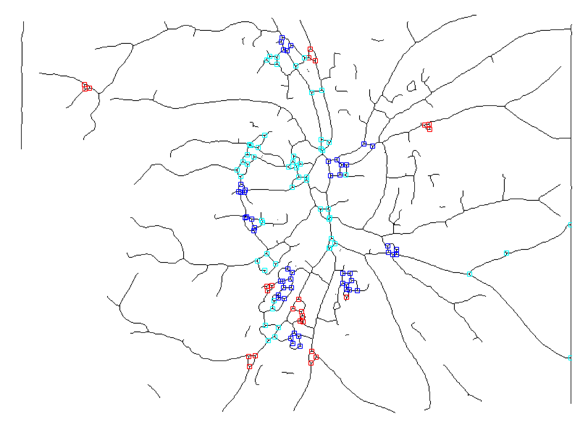
\includegraphics[width=0.5\linewidth]{345cycle.png}
  \caption{一幅视网膜图像的所有环结构图}
    \label{345cycle}
 \end{figure}

事实上“环”的概念来源于图论,在图论中,一个图$G$定义为一个有序对$G=(V,E)$,其中点集$V$是顶点的集合,$E$则是边的集合同时是$V$的二元子集,即一条边与两个顶点相连,并且这种连接关系被表达为对应特定边顶点的无序对。

下面是关于图的几个概念:

图可分为有向图和无向图:若一个图中每条边均有方向,称为有向图;若一个图中每条边都是无方向的,则称为无向图。

有权重图(赋权图)与无权重图:有权重图是每一条边均有权值的图,无权重图则为图的每一条边都不含有权值的图。

度(Degree):一个顶点的度是指与该顶点相关联的边的条数,顶点$v$的度记作$d(v)$。

顶点的邻接(Adjacent):对于无向图$G=(V,E)$,若顶点$V$和$W$之间至少有一条边相连,则称顶点$V$和$W$互为邻接点,即$V$和$W$相邻接。

在一个无向图$G$中,“环”指的是多个边的简单集合,其中“环”的每个顶点的度是偶数,而顶点的度等于与该顶点相连的边的个数。如果一组“环”组成了图$G$的环空间,那么这组环叫做图$G$的环基,即环基是图$G$的向量空间的基,在这个向量空间中,每组基向量代表一个简单环。一个图$G$的每个环基有相同数量的环,与它的环空间的维数相等。一个图$G$可以有多组环基,如果该图的一个环基它的所有环的权重的和最小,那么这个环基就称为图$G$的最小环基。在无权(重)图中,一个“环”的权重为环的边的数量。

图的最小环基在许多领域都有广泛的应用,如用于决定公共运输系统的行程安排~\cite{lieb},在生物学中用来从基因序列数据中决定单体型~\cite{derek},进行电力网络的分析,还可应用于结构工程,化学,平面重建等方面,因此成为众多学者研究的课题内容。

在视网膜图像中,视网膜血管网络可以看做一个无向无权图,血管的分叉点、交叉点为图的顶点,两个分叉点或交叉点之间的血管为边。我们定义的环结构则构成了视网膜血管图的最小环基,因此寻找环结构可以看做寻找视网膜血管图的最小环基。

\section{本章小结}
本章主要介绍了视网膜图像的预处理过程,主要包括多尺度分割,连通区域标记去噪,填充空洞和骨架化过程。重点讲述了连通区域标记的过程和轮廓修建骨架化过程。同时提出了多尺度的概念,通过控制视网膜血管图像下不同尺度的变化,得到存在不同细节程度的分割结果,与单一分割结果相比,避免了因单个分割结果失败造成后续的配准失败的情况,而且更有利于下步环结构的构建。

本章重点介绍了环结构的概念:环结构是由动脉和静脉的血管的分叉点、交叉点及相连接的血管组成的结构。阐述了图论中关于环的概念,并给出了寻找环结构就是寻找视网膜血管图的最小环基的推论。



